\begin{figure}[t]
	\centering
% 	\copyrightbox[r]{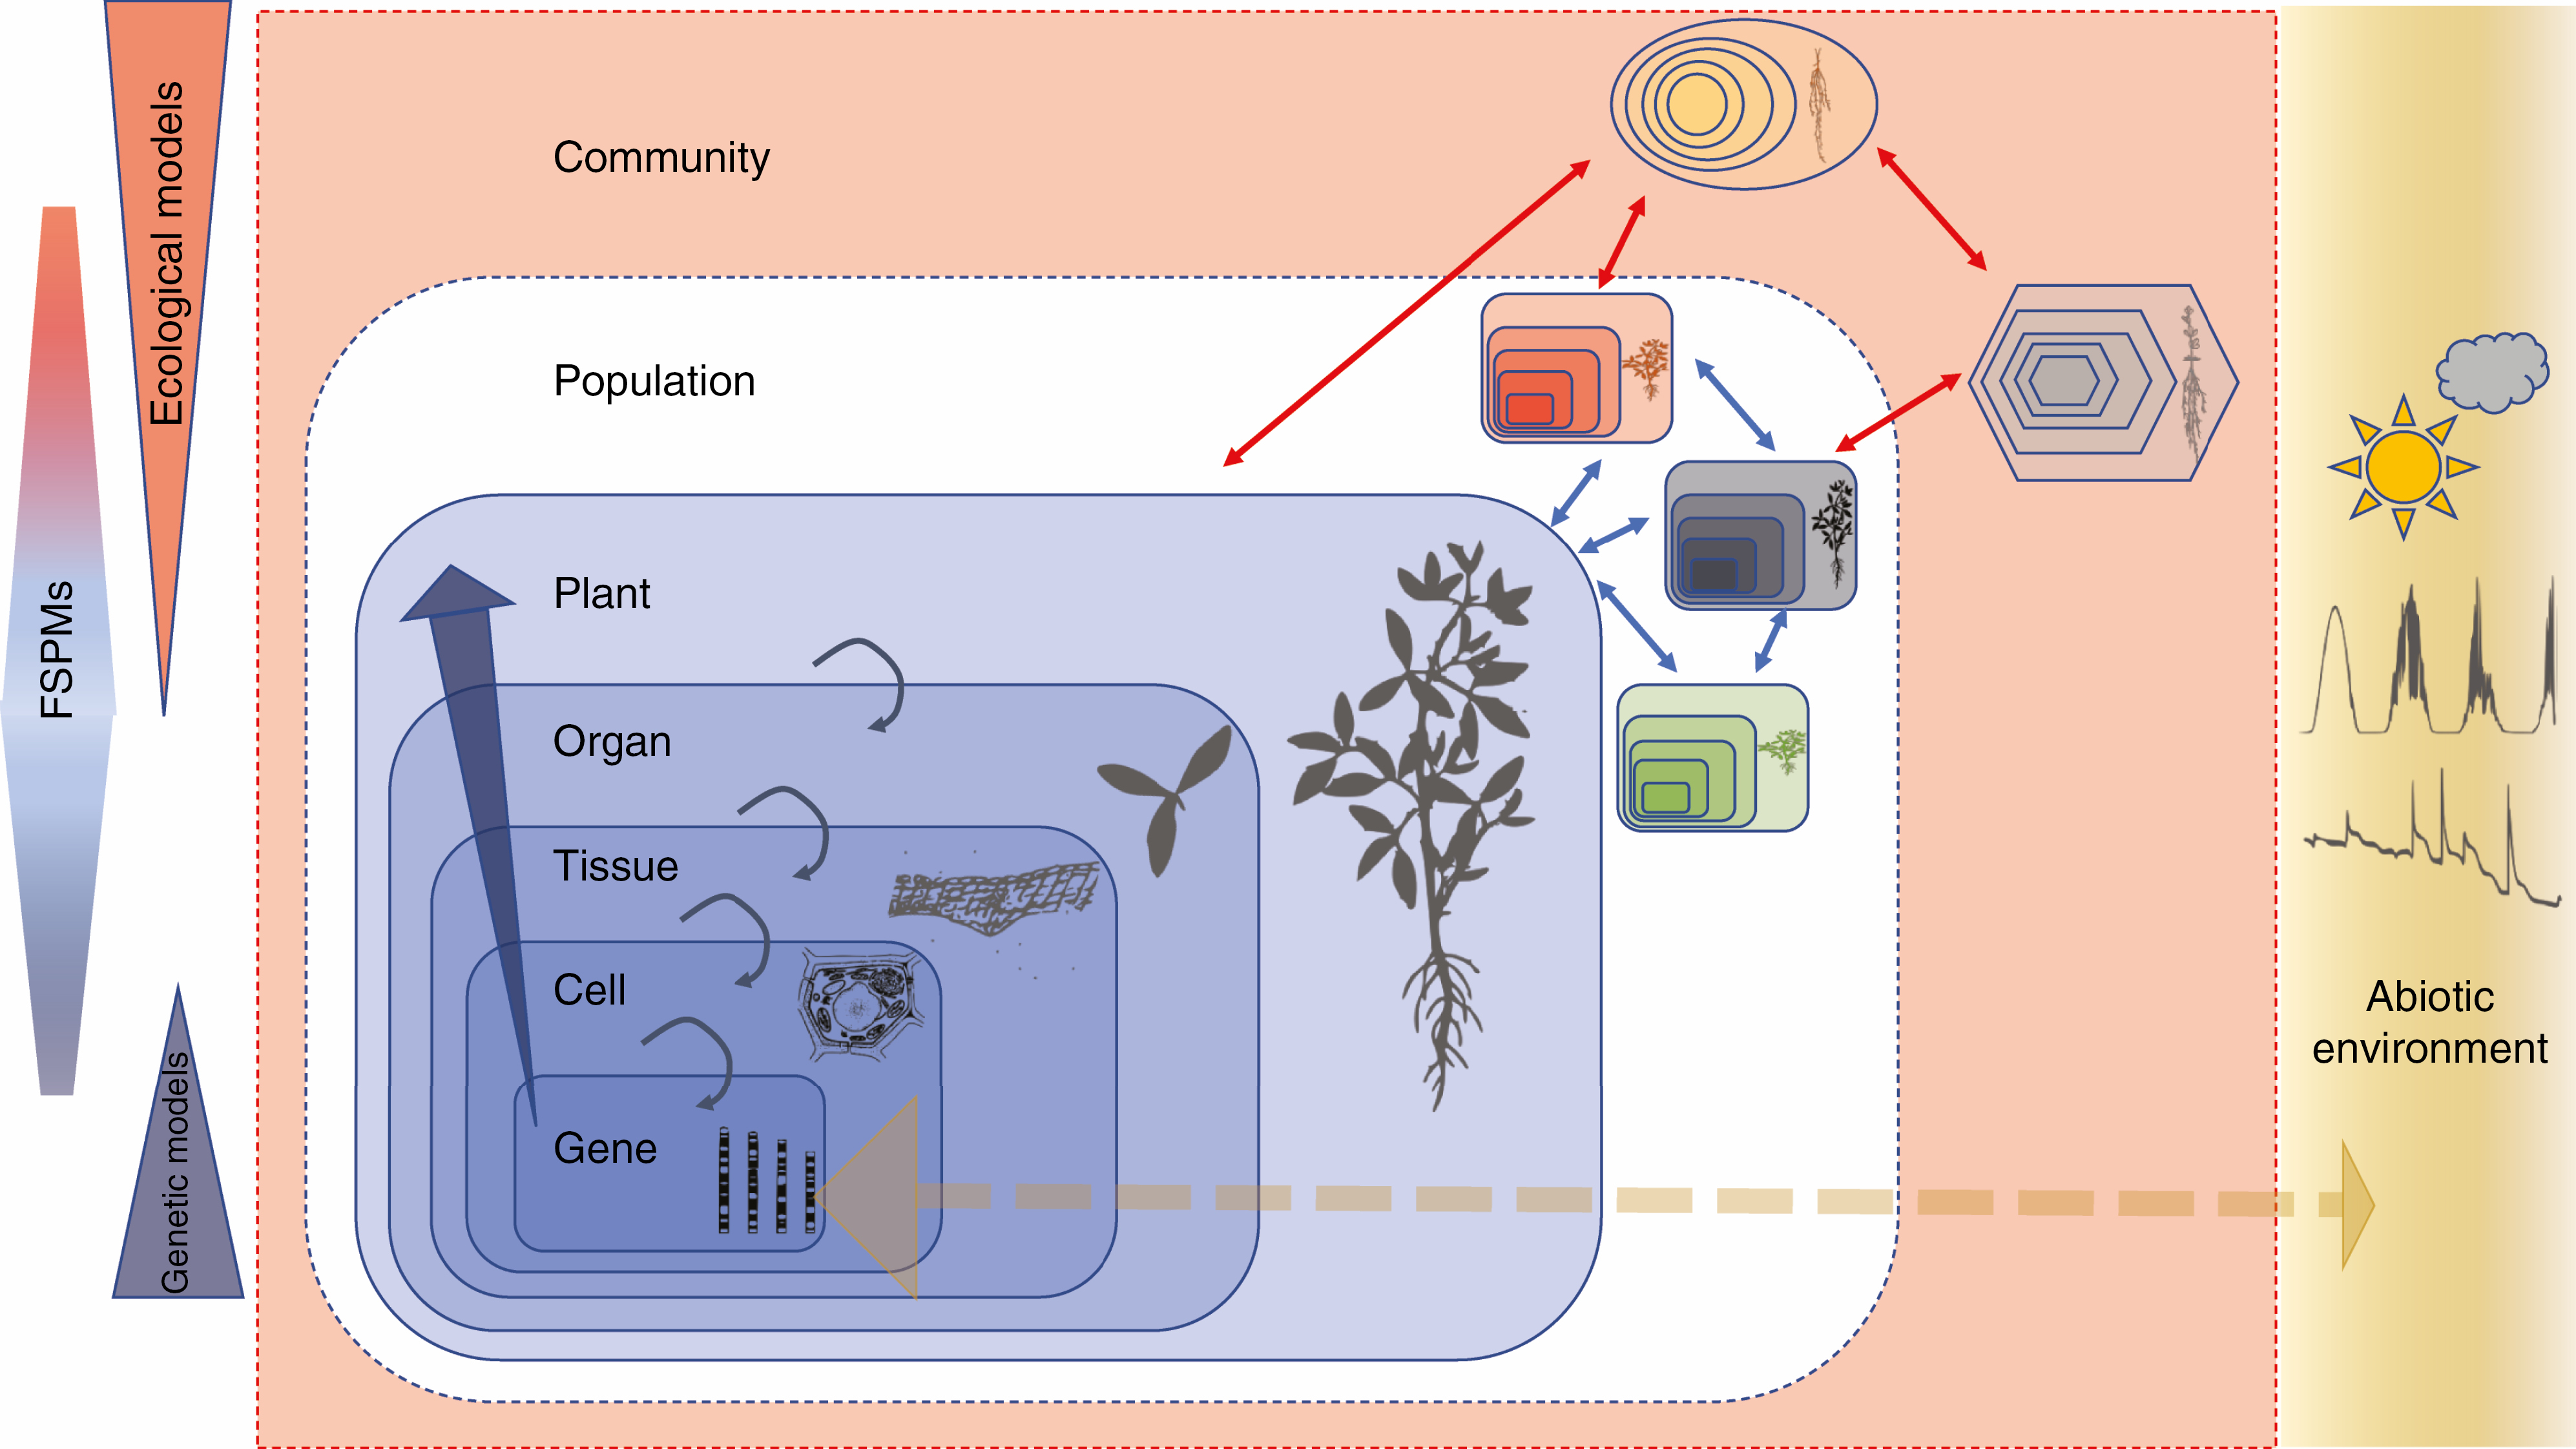
\includegraphics[width=0.8\textwidth]{img/fspm_scales_louarn_2020.jpeg}}{\textcopyright Copyright 2020 Oxford University Press}
	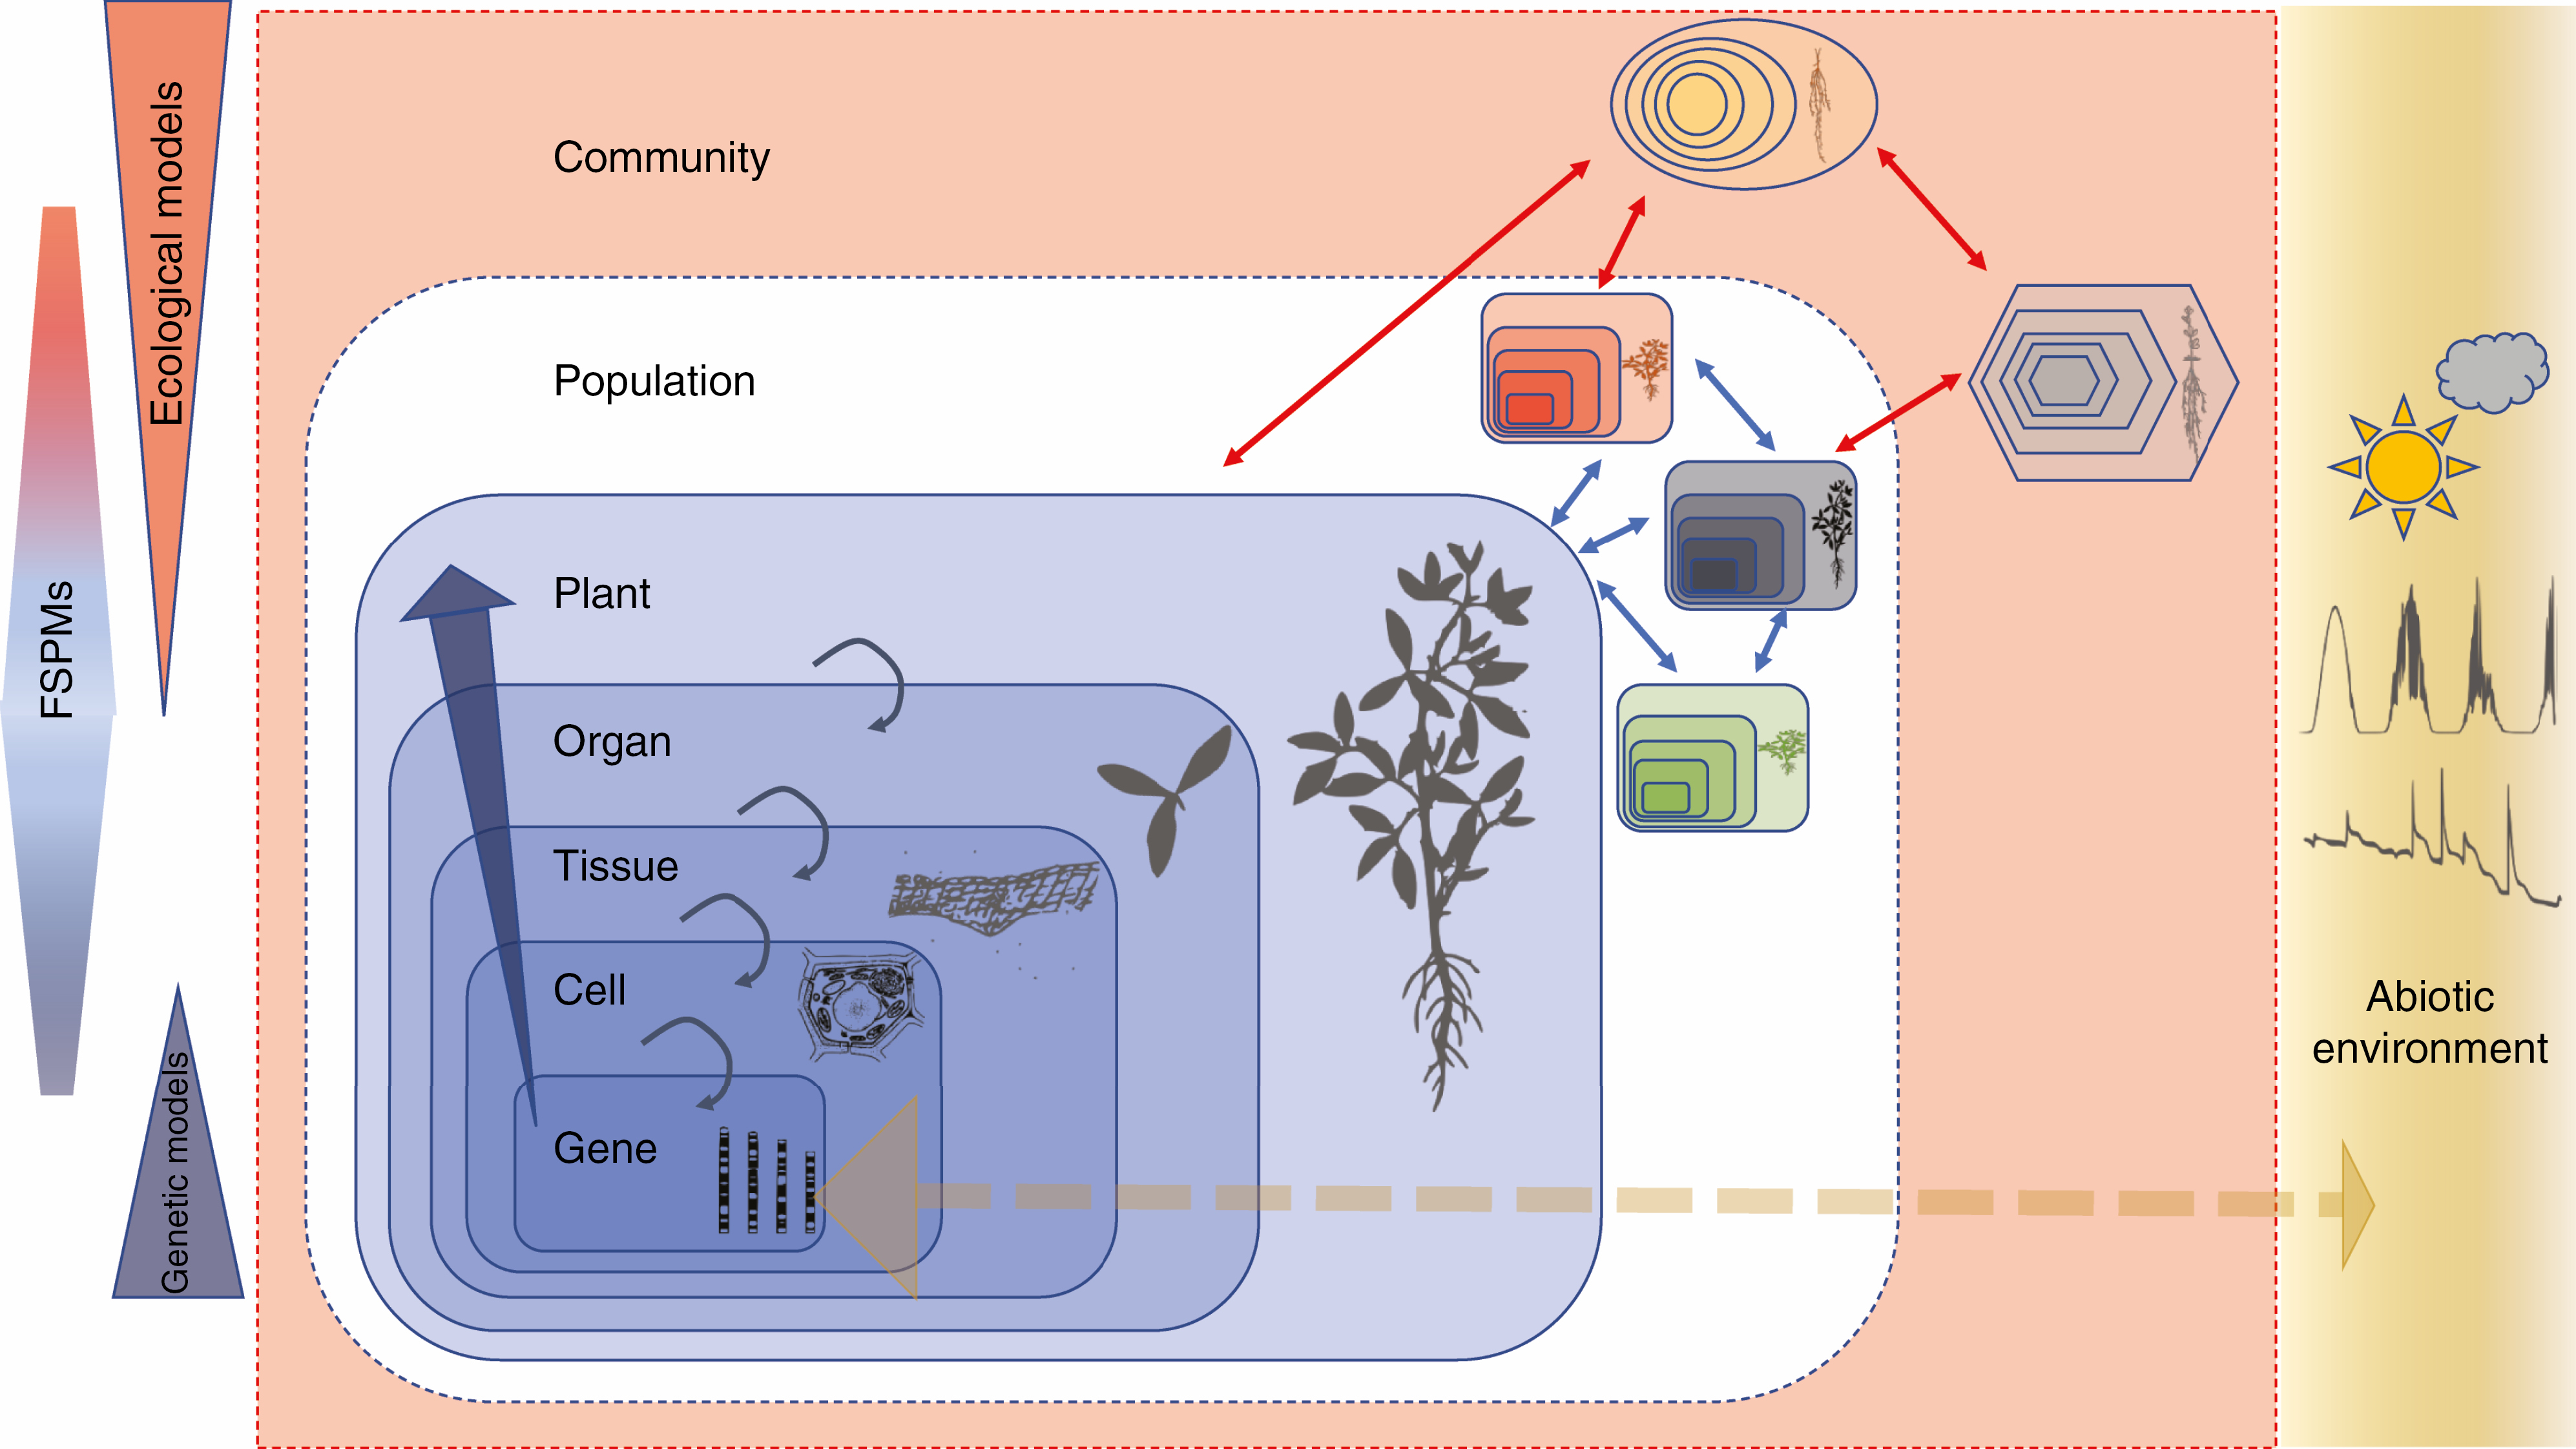
\includegraphics[width=\textwidth]{img/fspm_scales_louarn_2020.jpeg}
	
	\caption[Interactions at micro- and macroscopic scales present in functional-structural plant models (from \citet{louarn_two_2020}).]{
	        Interactions at micro- and macroscopic scales present in functional-structural plant models.
    	    \acrshort{fspm}s typically implement a subset of the scales depicted in the figure. The interactions between structural elements at one level govern the macroscopic behavior at the higher level. All levels interact with the environment. In some models, the behavior of the lowest level units is governed by variable genetic properties. This figure is reused from \citet{louarn_two_2020} with permission from the publisher.
        }
	\label{fig:fspm_scales_louarn2020}
\end{figure}


% Original caption:

% FSPMs cover a range of scale integration from gene to community level, with the focus of attention being the explanation of how plant phenotypes (centre of the figure) are built from interactions with their inner (including genetic determinants and self-regulation loops expressed at various levels) and outer (including abiotic factors and biotic interactions in plant populations and communities) environments. Interactions up to the plant scale involve sub-parts that all share the same genetic material (same shape and colour gradient in the figure) and proceed from systems biology. Interactions at higher scales integrate the interplay between entities that are genetically distinct (either from the same or different species), and contribute to predictive ecology by linking organismal traits with population and community functioning. FSPMs thus complete both classical genetic and molecular network models that are usually applied up to the cellular level, and population ecology models that are lacking a robust physiological response to environmental drivers.